\section{Extensions}
\label{sec:extensions}

\subsection{CPU-based Scatter-Gather DMA}

PCIe has 29\% TLP header and padding overhead for 64B DMA operations (\S\ref{sec:challenge}) and the DMA engine may not have enough parallelism to saturate the PCIe bandwidth-delay product with small TLPs (\S\ref{sec:implementation}).
Larger DMA operations with up to 256-byte TLP payload is supported by the PCIe root complex in our system. In this case, the TLP head and padding overhead is only 9\%, and the DMA engine has enough parallelism (64) to saturate the PCIe link with 27 in-flight DMA reads.
To batch the DMA operations on PCIe link, we can leverage the CPU to perform scatter-gather (Figure~\ref{fig:sg-arch}).
First, the NIC DMAs addresses to a request queue in host memory. The host CPU polls the request queue, performs random memory access, put the data in response queue and writes MMIO doorbell to the NIC. The NIC then fetches the data from response queue via DMA.

\begin{figure}[t]
\centering
\subfloat[Read.\label{fig:sge-read}]
{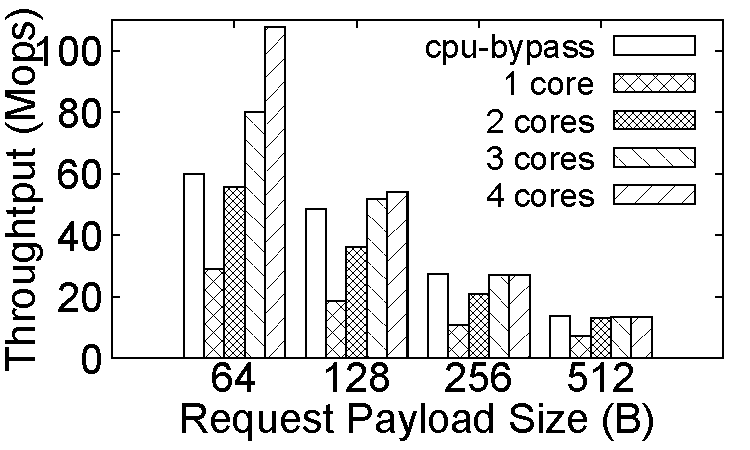
\includegraphics[width=.25\textwidth,page=1]{sg-read.pdf}}
\subfloat[Write.\label{fig:sge-write}]
{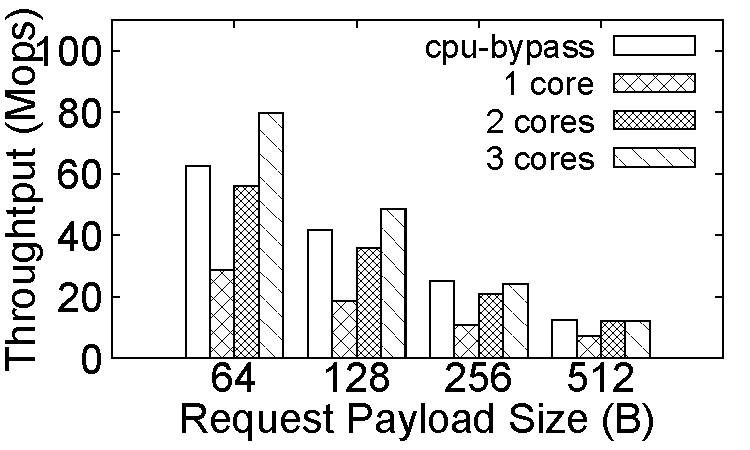
\includegraphics[width=.25\textwidth,page=1]{sg-write.pdf}}
\caption{Scatter-gather performance.}
\label{fig:scatter-gather}
\vspace{-15pt}
\end{figure}

Figure~\ref{fig:scatter-gather} shows that CPU-based scatter-gather DMA has up to 79\% throughput improvement compared to the CPU-bypassing approach.
In addition to the CPU overhead, the primary drawback of CPU-based scatter-gather is the additional latency.
To save MMIOs from the CPU to the NIC, we batch 256 DMA operations per doorbell, which requires 10~$\mu$s to complete.
The overall latency for the NIC to access host memory using CPU-based scatter-gather is \approx20~$\mu$s, almost 20x higher than direct DMA.

\subsection{Multiple NICs per Server}

\begin{figure}[t]
\begin{minipage}[t]{0.23\textwidth}
\centering
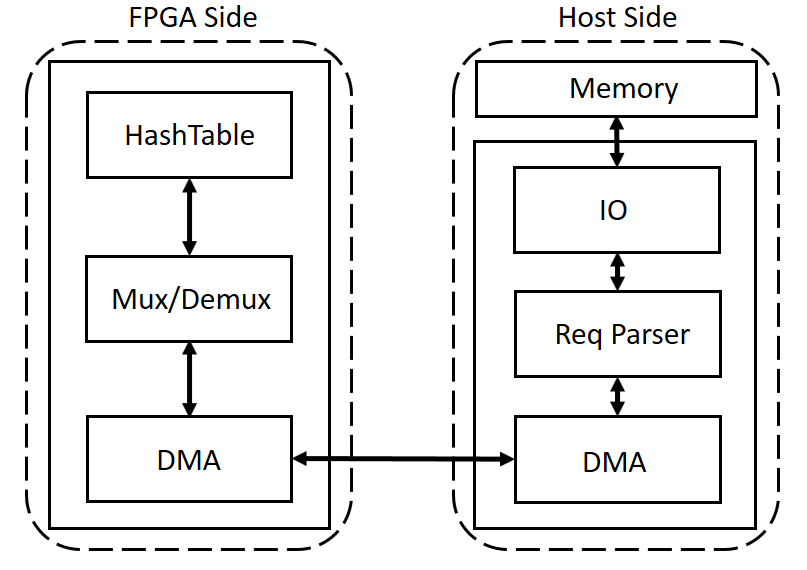
\includegraphics[width=1\textwidth,page=1]{scatter_gather.PNG}
\caption{Scatter-gather architecture.}
\label{fig:sg-arch}
\end{minipage}
\begin{minipage}[t]{0.23\textwidth}
\centering
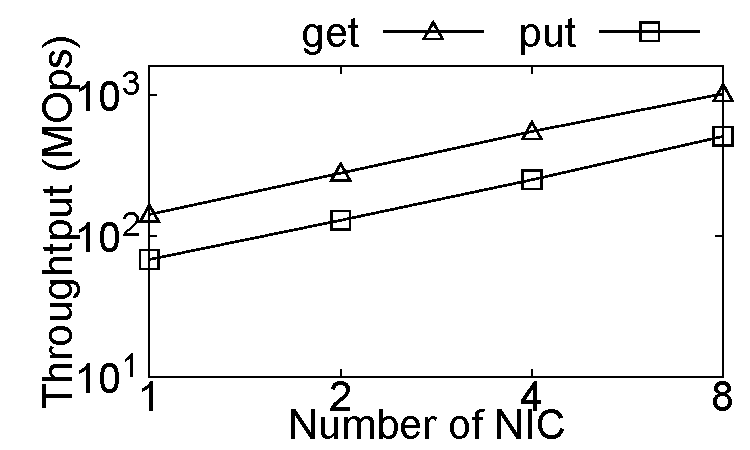
\includegraphics[width=1\textwidth,page=1]{multi_nic.pdf}
\caption{Performance of multiple NICs per server.}
\label{fig:multiple-nics}
\end{minipage}
\vspace{-10pt}
\end{figure}

%The primary use case for KV-Direct is to enable remote direct key-value access without CPU overhead on the server. 
In some cases, it may be desirable to build a dedicated key-value store with maximal throughput per server.
Through simulation, MICA~\cite{li2016full} showed the possibility of achieving a billion KV op/s in a single server with four (currently unavailable) 60-core CPUs.
As shown in Table~\ref{tab:kvs-compare}, with 8 KV-Direct NICs on a server, the one billion KV op/s performance is readily achievable with a commodity server and less than 400 watts of wall power.
The power efficiency for 8 NICs, however, is lower than single NIC, because we accounted for the power of host server.

Due to limited number of full-height PCIe slots in Dell R730 server, for multiple-NIC evaluation, we use an HPE Apollo 6500 server with 8 PCIe Gen3 x16 slots connected to two NUMA CPU nodes via 4 PLX PCIe switches.
Because the HPE server does not support PCIe bifurcation, only one PCIe Gen3 x8 is enabled on each NIC, so the throughput per NIC is lower than Figure~\ref{fig:ycsb-tput}.
Each NIC owns an exclusive memory region in host memory and serves a disjoint partition of keys.
Multiple NICs suffer the same load imbalance problem as a multi-core KVS implementation.
Fortunately, for a small number of partitions (e.g. 8), the load imbalance is not significant~\cite{li2016full}. Under YCSB long-tail workload, the highest-loaded NIC has 1.4x load of the average.
%In comparison, to achieve matching performance with 240 CPU cores, the load of the hottest core will be 10x of the average.
Figure~\ref{fig:multiple-nics} shows that KV-Direct throughput scales linearly with the number of NICs.
